\documentclass[notheorems]{beamer}

\usepackage{amsmath,amsthm,amssymb,setspace, mathtools}
\usepackage{physics}

\usepackage{color}   %May be necessary if you want to color links
\usepackage{hyperref}
\hypersetup{
	colorlinks=true, %set true if you want colored links
	linktoc=all,     %set to all if you want both sections and subsections linked
	linkcolor=black,  %choose some color if you want links to stand out
	urlcolor=cyan
}


%
%
%
\newif\ifhideproofs
%\hideproofstrue %uncomment to hide proofs
%
%
%
%
\ifhideproofs
\usepackage{environ}
\NewEnviron{hide}{}
\let\proof\hide
\let\endproof\endhide
\fi

\theoremstyle{definition}
\newtheorem{definition}{Definition}[subsection]
\newtheorem{defn}[definition]{Definition}
\newtheorem{nota}[definition]{Note}
\newtheorem{thm}[definition]{Theorem}
\newtheorem{lem}[definition]{Lemma}
\newtheorem{prop}[definition]{Proposition}
\newtheorem{cor}[definition]{Corollary}
\newtheorem{conj}[definition]{Conjecture}
\newtheorem{ex}[definition]{Exercise}
\newtheorem{ques}[definition]{Question}
\newtheorem{ans}[definition]{Answer}
\newtheorem{fact}[definition]{Fact}
\newtheorem{rem}[definition]{Remark}

\newcommand{\al}{\alpha}
\newcommand{\Gam}{\Gamma}
\newcommand{\be}{\beta} 
\newcommand{\del}{\delta} 
\newcommand{\Del}{\Delta}
\newcommand{\lam}{\lambda}  
\newcommand{\Lam}{\Lambda} 
\newcommand{\ep}{\epsilon}
\newcommand{\sig}{\sigma} 
\newcommand{\om}{\omega}
\newcommand{\Om}{\Omega}
\newcommand{\C}{\mathbb{C}}
\newcommand{\N}{\mathbb{N}}
\newcommand{\E}{\mathbb{E}}
\newcommand{\Z}{\mathbb{Z}}
\newcommand{\R}{\mathbb{R}}
\newcommand{\T}{\mathbb{T}}
\newcommand{\Q}{\mathbb{Q}}
\renewcommand{\P}{\mathbb{P}}
\newcommand{\MA}{\mathcal{A}}
\newcommand{\MC}{\mathcal{C}}
\newcommand{\MB}{\mathcal{B}}
\newcommand{\MF}{\mathcal{F}}
\newcommand{\MG}{\mathcal{G}}
\newcommand{\ML}{\mathcal{L}}
\newcommand{\MN}{\mathcal{N}}
\newcommand{\MS}{\mathcal{S}}
\newcommand{\MP}{\mathcal{P}}
\newcommand{\ME}{\mathcal{E}}
\newcommand{\MT}{\mathcal{T}}
\newcommand{\MM}{\mathcal{M}}
\newcommand{\MI}{\mathcal{I}}

\newcommand{\ui}{[0,1]}
\newcommand{\p}{\partial}

\newcommand{\io}{\text{ i.o.}}
%\newcommand{\ev}{\text{ ev.}}
\renewcommand{\r}{\rangle}
\renewcommand{\l}{\langle}

\newcommand{\RG}{[0,\infty]}
\newcommand{\Rg}{[0,\infty)}
\newcommand{\Ru}{(\infty, \infty]}
\newcommand{\Rd}{[\infty, \infty)}
\newcommand{\Ll}{L^1_{\text{loc}}(\R^n)}

\newcommand{\limfn}{\liminf \limits_{n \rightarrow \infty}}
\newcommand{\limpn}{\limsup \limits_{n \rightarrow \infty}}
\newcommand{\limn}{\lim \limits_{n \rightarrow \infty}}
\newcommand{\convt}[1]{\xrightarrow{\text{#1}}}
\newcommand{\conv}[1]{\xrightarrow{#1}} 
\newcommand{\seq}[2]{(#1_{#2})_{#2 \in \N}}

\newcommand{\lsc}{l.s.c. }

\DeclareMathOperator{\supp}{supp}
\DeclareMathOperator{\sgn}{sgn}
\DeclareMathOperator{\spn}{span}
\DeclareMathOperator{\iso}{Iso}
\DeclareMathOperator{\id}{id}
\DeclareMathOperator*{\argmax}{arg\,max}
\DeclareMathOperator*{\argmin}{arg\,min}


%Information to be included in the title page:
\title{Approximating Posterior Gaussian Processes}
\author{Carson James}

\begin{document}

\frame{\titlepage}

\begin{frame}
\frametitle{Outline}
\tableofcontents
	
\end{frame}

%\begin{enumerate}
%	\item Banach Spaces
%		\begin{itemize}
%		\item bounded linear maps
%		\item Frechet differentiation
%		\end{itemize}
%	\item Calculus 
%		\begin{itemize}
%		\item tools
%		\item results
%		\end{itemize}
%	\item Hilbert Spaces
%		\begin{itemize}
%		\item Riesz representation theorem
%		\item gradients
%		\end{itemize}
%	\item Convex Analysis 
%		\begin{itemize}
%		\item results for Frechet differentiable functions
%		\end{itemize}
%	\item Reproducing Kernel Hilbert Spaces
%		\begin{itemize}
%		\item representer theorem
%		\end{itemize}
%	\item Applications to Gaussian Processes
%	\begin{itemize}
%		\item predictive posterior 
%		\end{itemize}
%	
%	\end{enumerate}

\section{Gaussian Processes}

\begin{frame}
\frametitle{Gaussian Processes}

\begin{nota}
Let $T$ be a set, $f:T \rightarrow \R$, $\mu: T \rightarrow \R$, $c: T^2 \rightarrow \R$, $x = (x_j)_{j=1}^n \in T^n$ and $t \in T$. 
We will write 
\begin{itemize}
\item $f(x) \coloneqq (f(x_j))_{j =1}^n \in \R^n$
\item $\mu(x) \coloneqq (\mu(x_j))_{j =1}^n \in \R^n$ 
\item $c(x, x) \coloneqq (c(x_i, x_j))_{i,j} \in \R^{n \times n}$
\item $c(x, t) \coloneqq (c(x_j, t))_{i,j} \in \R^{n \times 1}$
\item $c(t, x) \coloneqq (c(t, x_j))_{i,j} \in \R^{1 \times n}$
\end{itemize}

\end{nota}

\begin{defn}
Let $T$ be a set and $c: T^2 \rightarrow \R$. Then $c$ is said to be \textbf{positive definite} if for each $(x_j)_{j=1}^n \in T^n$, the matrix $c(x,x)$ is positive definite. 
\end{defn}

\end{frame}









\begin{frame}
\frametitle{Gaussian Processes}

\begin{defn}
Let $T$ be a set, $(\Om, \MF, P)$ a probability space, $\mu : T \rightarrow \R$, $c: T^2 \rightarrow \R$ symmetric and positive definite and $f: T \rightarrow L^2(\Om, \MF, P)$ (i.e. $f$ is a random function from $T$ to $\R$). Then $f$ is said to be a \textbf{Gaussian Process} with mean function $\mu$ and covariance function $c$, denoted $f \sim GP(\mu, c)$, if for each $x = (x_j)_{j=1}^n \in T^n$, $f(x) \sim N_{n}(\mu(x), c(x,x))$. 
\end{defn}
\end{frame}
















\begin{frame}
\frametitle{Gaussian Processes}

\begin{fact}
Let $T$ be a set, $c: T^2 \rightarrow \R$ positive definite, $x = (x_j)_{j=1}^n \in T^n$, $y = (y_j)_{j=1}^n \in \R^n$. Suppose we have the following model:
\begin{align*}
y_i &= f(x_i) + \ep_i \\
\ep_i &\sim N(0, \sig^2) \\
f &\sim GP(0, c)
\end{align*}
Then $$f|x, y \sim GP(\tilde{\mu}, \tilde{c})$$ where $$\tilde{\mu}(t) = c(t, x)[c(x,x) + \sig^2I]^{-1}y$$ and $$\tilde{c}(s,t) = c(s,t) - c(s,x)[c(x,x) + \sig^2 I]^{-1}c(x,t)$$

\end{fact}
\end{frame}














\begin{frame}
\frametitle{Gaussian Processes}

\begin{ques}
Suppose that we want to evaluate $\tilde{\mu}(t) = c(t, x)[c(x,x) + \sig^2I]^{-1}y$ and $\tilde{c}(s,t) = c(s,t) - c(s,x)[c(x,x) + \sig^2 I]^{-1}c(x,t)$ for many input values of $(s,t)$. \\
What do we do when $[c(x,x) + \sig^2 I]^{-1}$ is too expensive to compute, or perhaps computable after a fair bit of time, but finding the values $\tilde{c}(s,t)$ repeadtedly for many inputs of $(s,t)$ is not feasible? 
\end{ques}

\pause
\begin{ans}
One thing to try would be to approximate $\tilde{\mu}$ and $\tilde{c}$. In this case we discuss approximating $\tilde{\mu}$ and $\tilde{c}$ with neural networks. Then, after training, evaluation would be constant time (with respect to data size).
\end{ans}

\end{frame}
















\begin{frame}
\frametitle{Gaussian Processes}

\begin{ques}
If we want to approximate $\tilde{\mu}$ and $\tilde{c}$ with neural networks, we need a loss function to train the networks. What should this loss function be? 
\end{ques}

\pause
\begin{ans}
We propose using a loss function derived from an alternative formulation of the posterior mean and covariance. To make this less vague, we will discuss the necessary background, which consists of calculus on Banach spaces and convex analyis on Banach spaces and repoducing kernel Hilbert spaces .
\end{ans}

\end{frame}







\section{Banach Spaces}


\begin{frame}
\frametitle{Banach Spaces}
	
	\begin{rem}
	When working with finite dimensional normed vector spaces, all linear operators are continuous. However, in general this is not true if we drop the assumption of finite dimensionality. We will introduce the concept of boundedness, which is equivalent to continuity in the context of linear operators.
	\end{rem}	
	
	\end{frame}
	
	
	
	
	
	
	
	
	
	
	
	
	
	
	
	
	\begin{frame}
	\frametitle{Banach Spaces}
	
	\begin{defn}
		Let $X,Y$ be a normed vector spaces and $T:X \rightarrow Y$ a linear map. Then $T$ is said to be \textbf{bounded} if there exists $C \geq 0$ such that for each $x \in X$, $$\|Tx \|\leq C \|x \|$$ We define $$L(X;Y) = \{T:X \rightarrow Y: T \text{ is linear and bounded}\}$$
	\end{defn}
	
	\pause
	\begin{defn}
	Let $X$ be a normed vector space over $\R$. We define the \textbf{dual space of} $X$, denoted $X^*$, by $X^* = L(X; \R)$. Let $T: X \rightarrow \R$. Then $T$ is said to be a \textbf{bounded linear functional on} $X$ if $T \in X^*$.
	\end{defn}
	\end{frame}
	
	
	
	
	
	
	
	
	
	
	
	
	
	
	
	
	
	
	
	\begin{frame}
	\frametitle{Banach Spaces}
	
	\begin{defn}
		Let $X_1, \dots, X_n$ and $Y$ be a normed vector spaces and $T:\prod\limits_{j=1}^n X_j \rightarrow Y$ a multilinear linear map. Then $T$ is said to be \textbf{bounded} if there exists $C \geq 0$ such that for each $(x_j)_{j=1}^n \in \prod\limits_{j=1}^n X_j$, $$\|T(x_1, \dots, x_n) \|\leq C \|x_1 \| \dots \|x_n\|$$ 
		We define $$L^n(X_1, \dots, X_n; Y) = \{T:X \rightarrow Y: T \text{ is multilinear and bounded}\}$$ 
		If $X_1, \dots, X_n = X$, we write $L^n(X;Y)$ in place of  $L^n(X, \dots, X; Y)$.
	\end{defn}
	
	\end{frame}
	
	
	
	
	
	

	
	
	
	
	
	
	
	
	
	
	
	
	
	
	
	
	\begin{frame}
	\frametitle{Banach Spaces}
	
	\begin{defn}
	Let $X$ and $Y$ be normed vector spaces. We define the \textbf{operator norm}, denoted $\|\cdot\|: L^2(X;Y) \rightarrow [0, \infty)$ by $$\|T\| = \inf \{C \geq 0: \text{for each } (x_1, x_2) \in X^2 \text{, } \|T(x_1, x_2) \|\leq C\|x_1\|\|x_2\|\}$$
	\end{defn}
	
	
	\pause
	\begin{fact}
	Let $X$ and $Y$ be normed vector spaces. Then $\|\cdot\|: L^2(X;Y) \rightarrow [0, \infty)$ is a norm.
	\end{fact}
	
	
	\pause
	\begin{rem}
	Let $X$ and $Y$ be normed vector spaces. We may identify $L(X; L(X;  Y))$ and $L^2(X; Y)$ via the isometric isomorphism $L(X; L(X;  Y)) \rightarrow L^2(X;Y)$ given by $\phi \mapsto \psi_{\phi}$ where $$\psi_{\phi}(x_1, x_2) = \phi(x_1)(x_2)$$ 
	This immediately generalizes to higher dimensions.
	\end{rem}

	\end{frame}
	
	
	
	
	
	
	
	
	






\begin{frame}
\frametitle{Banach Spaces}



	\begin{rem}
	To discuss differentiation on normed vector spaces, we need to be able to talk about limits. Assuming completeness lets us do just this. 
	\end{rem}
	
	\pause
\begin{defn}
		Let $X$ be a normed vector space. Then $X$ is said to be a \textbf{Banach space} if $X$ is complete.  
	\end{defn}
	
	
\end{frame}







































\begin{frame}
	\frametitle{Banach Spaces}
	

	\begin{defn}
	Let $X, Y$ be a banach spaces, $A \subset X$ open, $f:A \rightarrow Y$ and $x_0 \in A$. Then $f$ is said to be \textbf{\textbf{($1$-st order) Frechet differentiable} at $x_0$} if there exists $Df(x_0) \in L(X;Y)$ such that, $$f(x_0 + h) = f(x_0) + Df(x_0)(h) + o(\|h\| ) \hspace{.5cm} \text{ as } h \rightarrow 0$$  
	If $f$ is Frechet differentiable at $x_0$, we define the \textbf{Frechet derivative of $f$ at $x_0$} to be $Df(x_0)$.
	We say that $f$ is \textbf{($1$-st order) Frechet differentiable} if for each $x_0 \in A$, $f$ is Frechet differentiable at $x_0$. \\
	If $f$ is Frechet differentiable, we define the \textbf{($1$-st order) Frechet derivative} of $f$, denoted $Df: A \rightarrow L(X;Y)$, by $$x \mapsto Df(x)$$
	
	\end{defn}

\end{frame}































\begin{frame}
\frametitle{Banach Spaces}


\begin{defn}
Continuing inductively, if $f$ is $(n-1)$-th order Frechet differentiable, $f$ is said to be \textbf{$n$-th order Frechet differentiable at $x_0$} if $D^{n-1}f$ is Frechet differentiable at $x_0$. We define $D^nf(x_0) = D(D^{n-1}f)(x_0)$.
If $f$ is $n$-th order Frechet differentiable, we define the \textbf{($n$-th) order Frechet derivative} of $f$, denoted $D^nf: A \rightarrow L^n(X;Y)$, by $$x \mapsto D^nf(x)$$
\end{defn}

\begin{rem}
Using the identification mentioned earlier, we may think of the $n$-th Frechet derivative as a bounded multilinear map:  $D^nf(x_0) \in L^n(X;Y)$. 
\end{rem}


\end{frame}








\begin{frame}
\frametitle{Banach Spaces}

\begin{rem}
The tools used to obtain the following results: 
\begin{itemize}
\item Frechet Derivative
\item Bochner Integral
\item Hahn-Banach Theorem  
\end{itemize}
\end{rem}

\begin{fact}
Let $X,Y$ be Banach spaces and $f \in L(X;Y)$. Then $f$ is Frechet differentiable and for each $x_0 \in X$, $Df(x_0) = f$. 
\end{fact}
\pause

\begin{fact}
Let $X,Y, Z$ be Banach spaces, $f:X \rightarrow Y$, $g :Y \rightarrow Z$ and $x_0 \in X$. If $f$ is Frechet differentiable at $x_0$ and $g$ is Frechet differentiable at $f(x_0)$, then $g \circ f$ is Frechet differentiable at $x_0$ and $$D(g \circ f)(x_0) = Dg(f(x_0)) \circ Df(x_0)$$
\end{fact}
\pause

\begin{fact}
Let $X, Y$ be a Banach spaces, $A \subset X$ open and convex and $f:A \rightarrow Y$. If $f$ is Frechet differentiable, then for each $x,y \in A$, there exists $t \in (0,1)$ such that $$\|f(x) - f(y)\| \leq \|Df(tx + (1-t)y)\|\|x-y\|$$
\end{fact}


\end{frame}















\begin{frame}
\frametitle{Banach Spaces}

\begin{fact}
Let $X, Y$ be a Banach spaces, $A \subset X$ open and convex and $f:A \rightarrow Y$. Suppose that $f$ is Frechet differentiable. If for each $x \in A$, $Df(x) = 0$, then $f$ is constant.
\end{fact}
\pause

\begin{fact}
Let $X, Y$ be a Banach spaces, $A \subset X$ open and convex and $f,g:A \rightarrow Y$. Suppose that $f$ and $g$ are Frechet differentiable. If $Df = Dg$, then there exists $c \in Y$ such that $f = g+c$.
\end{fact}
\pause

\begin{fact}
Let $X$ be a Banach spaces, $A \subset X$ open, $f:A \rightarrow \R$ and $x_0 \in A$. Suppose that $f$ is Frechet differentiable at $x_0$. If $f$ has a local minimum at $x_0$, then $Df(x_0) = 0$. 
\end{fact}
\end{frame}












\begin{frame}
\frametitle{Banach Spaces}

\begin{fact}
Let $Y$ be a separable Banach space and $f \in C^1_Y(a,b)$. Then for each $x, x_0 \in (a,b)$, $x_0 < x$ implies that 
	\begin{enumerate}
	\item $f'$ is Bochner integrable on $(x_0, x]$ 
	\item  $$f(x) - f(x_0) = \int_{(x_0, x]}f'dm$$ 
	\end{enumerate}
\end{fact}
\pause

\begin{fact}
Let $Y$ be a separable Banach space, $A \subset X$ open and convex, $f\in C^n_Y(A)$ and $x_0 \in A$. Then $$f(x_0 + h) = \sum_{k=0}^n \frac{1}{k!} D^k f(x_0)(h, \dots, h) + o(\|h\|^n) \hspace{1cm }\text{ as } h \rightarrow 0$$
\end{fact}
\end{frame}


















\section{Convex Analysis}

\begin{frame}
\frametitle{Convex Analysis}


\begin{defn}
Let $X$ be a vector space, $A \subset X$ convex, $f:A \rightarrow \R$ convex and $x_0 \in A$. Then $f$ is said to be \textbf{convex} if for each $t \in [0,1]$ and $x,y \in A$, $$f(tx + (1-t)y) \leq tf(x) + (1-t)f(y)$$
\end{defn}

\pause
\begin{fact}
Let $X$ be a vector space, $A \subset X$ convex, $f:A \rightarrow \R$ convex and $x_0 \in A$. Then $f$ has a local minimum at $x_0$ iff $f$ has a global minimum at $x_0$.
\end{fact}

\pause
\begin{fact}
Let $X$ be a vector space, $A \subset X$ convex and $f:A \rightarrow \R$ strictly convex. If $f$ has a local minimum, then there exists a unique $x_0 \in A$ such that $f(x_0) = \min\limits_{x \in A}f(x)$.
\end{fact}



\end{frame}


















\begin{frame}
\frametitle{Convex Analysis}


\begin{fact}
Let $X$ be a Banach space, $A \subset X$ open and convex, $f:A \rightarrow \R$ convex, $x_0 \in A$. Suppose that $f$ is $2$nd order Frechet differentiable. Then $f$ is convex iff for each $x_0 \in A$, $D^2f(x_0)$ is positive semidefinite. 
\end{fact}

\begin{rem}
By positive semidefinite, we mean $D^2f(x_0)(h,h) \geq 0$ for $h \neq 0$.
\end{rem}


\pause
\begin{fact}
Let $X$ be a Banach space, $A \subset X$ open and convex, $f:A \rightarrow \R$ convex, $x_0 \in A$. Suppose that $f$ is $2$nd order Frechet differentiable. If for each $x_0 \in A$, $D^2f(x_0)$ is positive  definite, then $f$ is strictly convex. 
\end{fact}
\end{frame}






\section{Reproducing Kernel Hilbert Spaces}
\begin{frame}
\frametitle{Reproducing Kernel Hilbert Spaces}



\begin{defn}
Let $H$ be an inner product space. Then $H$ is said to be a \textbf{Hilbert space} if $H$ is complete with respect to the norm induced by the inner product.
\end{defn}
\pause

\begin{rem}
We will be assuming the Hilbert space is real. 
\end{rem}
\pause

\begin{fact}
Let $H$ be an inner product space. Then for each $x,y \in H$, $|\l x, y\r| \leq \|x\| \|y\|$ with equality iff $x \in \spn(y)$.
\end{fact}
\end{frame}


















\begin{frame}
\frametitle{Reproducing Kernel Hilbert Spaces}

\begin{defn}
Let $H$ be a Hilbert space. Define $\phi:H \rightarrow H^*$ by $x \mapsto x^*$ where $$x^*y = \l x ,y\r$$
\end{defn}
\pause

\begin{fact}
Let $H$ be a Hilbert space. Then $\phi: H \rightarrow H^*$ defined above is an isometric isomorphism.
\end{fact}

\end{frame}


















\begin{frame}
\frametitle{Reproducing Kernel Hilbert Spaces}

\begin{defn}
Let $H$ be a Hilbert space, $f: H \rightarrow \R$ and $x_0 \in H$. Suppose that $f$ is Frechet differentiable at $x_0$ so that $Df(x_0) \in H^*$. We define the \textbf{gradient of $f$ at $x_0$}, denoted $\nabla f(x_0) \in H$, by $$\nabla f(x_0) = Df(x_0)^*$$ That is, $\nabla f(x_0)$ is the unique element of $H$ such that for each $y \in H$, $$\l \nabla f(x_0), y \r = Df(x_0)(y)$$
\end{defn}


%
%\begin{fact}
%Let $H$ be a Hilbert space, $f:H \rightarrow \R$ and $x_0 \in H$. If $f$ is Frechet differentiable at $x_0$, %then 
%$$\argmin_{\|h\| \leq 1} Df(x_0)(h) = - \|\nabla f(x_0)%\|^{-1} \nabla f(x_0)$$ 
%\end{fact} 
%
\end{frame}



















\begin{frame}

\frametitle{Reproducing Kernel Hilbert Spaces}



\begin{defn}
Let $T$ be a set and $H \subset \R^T$ a hilbert space. For $t \in T$, we define the \textbf{evaluation functional at $t$}, denoted $l_t : H \rightarrow \R$, by $$l_t(f) = f(t)$$ 
\pause
The space $H$ is said to be a \textbf{reproducing kernel Hilbert space (RKHS)} if for each $t \in T$, $l_t \in H^*$ (i.e. $l_t$ is bounded). \\
\pause
If $H$ is an RKHS, the Riesz representation theorem implies that for each $t \in T$, there exists $c_t \in H$ such that for each $f \in H$, $\l c_t, f\r = f(t)$. \\
\pause
If $H$ is an RKHS, we define the \textbf{reproducing kernel} associated to $H$, denoted $c_H:T^2 \rightarrow \R$, by $$c_H(s,t) = \l c_s, c_t \r$$ 
\end{defn}
\end{frame}















\begin{frame}
\frametitle{Reproducing Kernel Hilbert Spaces}
\begin{fact}
Let $T$ be a set and $c : T^2 \rightarrow \R$. If $c$ is symmetric and positive definite, then there exists a unique reproducing kernel Hilbert space $H \subset \R^T$ such that $c_H = c$.
\end{fact}

\end{frame}









\begin{frame}
\frametitle{Reproducing Kernel Hilbert Spaces}
\begin{fact}
Let $T$ be a set, $c : T^2 \rightarrow \R$ a symmetric, postivie definite kernel on $T$, $H \subset \R^T$ the corresponding RKHS, $x = (x_j)_{j=1}^n \in T^n$, $\lam > 0$ and $y = (y_j)_{j=1}^n \in \R^n$. \\
\pause

Define $L_{\lam, y}: H \rightarrow \R$ by $$L_{\lam, y}(f) = \sum_{j=1}^n (y_j - f(x_j) )^2 + \lam \|f\|_H^2$$ \\
\pause 

Put $\hat{f} = \argmin\limits_{f \in H}L_{\lam, y}(f)$. 
\\
\pause 

Then there exist $(\hat{\al}_j)_{j=1}^n \subset \R$ such that $$\hat{f}(t) = \sum_{j=1}^n \hat{\al}_jc(t, x_j)$$
\end{fact}
\end{frame}















\begin{frame}
\frametitle{Reproducing Kernel Hilbert Spaces}
\begin{rem}
Recall that we defined $c(x,x) \in \R^{n \times n}$ by $c(x,x)_{i,j} = c(x_i, x_j)$. Some regular calculus shows that $\hat{\al} = (c(x,x) + \lam I)^{-1}y$.\\
Another way to write this is 
$$\hat{f}(t) = c(t,x)(c(x,x) + \lam I)^{-1}y$$
\end{rem}

\begin{rem}
Hopefully this looks familiar. Indeed, $\hat{f}$ is the posterior mean function of $f|x,y$ from our original model when $\lam = \sig^2$.
\end{rem}

\end{frame}















\begin{frame}
\frametitle{Reproducing Kernel Hilbert Spaces}
\begin{rem}
Define $Q: H \rightarrow \R$ by $$Q(f) = \sum_{j=1}^n (y_j - f(x_j) )^2$$ 
\pause
We can write rewrite $Q(f)$ as  $$Q(f) = \|l_x(f) - y\|_2^2$$ where $l_x \in L(H; \R^n)$ is given by $$l_x(f) = (f(x_j))_{j=1}^n$$ 
\end{rem}
\end{frame}












\begin{frame}
\frametitle{Reproducing Kernel Hilbert Spaces}
\begin{rem}
Writing this out, we see that 
\begin{align*}
Q(f_0 + h) 
&= \|l_x(f_0) - y\|_2^2  + 2(l_x(f_0) - y)^T l_x(h) + \|l_x(h)\|_2^2 \\
&= Q(f_0) + [\text{lin funct of $h$}] +  [\text{bilin funct of $(h,h)$}]
\end{align*}
\pause
Equating terms from Taylor's theorem, we see that $D^2Q(f_0)(h,h) = 2\|l_x(h)\|_2^2$, which is p.s.d. So $Q$ is convex. Since $\|f_0\|^2_H = \l f_0, f_0\r$ and $\l \cdot, \cdot \r$ is a positive definite bounded bilinear function on $H \times H$, $\|\cdot\|_H$ is strictly convex. Since $\lam > 0$, $L$ is strictly convex. 
\end{rem}
\end{frame}














\begin{frame}
\frametitle{Reproducing Kernel Hilbert Spaces}
\begin{rem}
Similar to before, writing out $L(f_0 + h)$, we get
$$L_{\lam, y}(f_0 + h) = L_{\lam, y}(f_0) + 2(l_x(f_0) - y)^T l_x(h) + 2 \lam \l f_0 , h\r + o(\|h\|^2) $$
\pause
So 
\begin{align*}
DL_{\lam, y}(f_0)(h) 
&= 2(l_x(f_0) - y)^T l_x(h) + 2 \lam \l f_0 , h\r \\
&= 2\sum_{j=1}^n (f_0(x_j)- y_j) \l c_{x_j}, h\r +  2 \lam \l f_0 , h\r \\
&= \bigg \l  2\bigg [ \sum_{j=1}^n (f_0(x_j)- y_j) c_{x_j} + \lam f_0\bigg ] , h \bigg \r 
\end{align*}
\pause
Hence $$\nabla L_{\lam, y}(f_0) = 2\bigg [ \sum_{j=1}^n (f_0(x_j)- y_j) c_{x_j} + \lam f_0\bigg ]$$
\end{rem}
\end{frame}















\section{Approximating Posterior Gaussian Processes}
\begin{frame}
\frametitle{Approximating Posterior Gaussian Processes}
\begin{rem}
Recall our model: Let $T$ be a set and $x = (x_j)_{j=1}^n \in T^n$, $y = (y_j)_{j=1}^n \in \R^n$. Recall that if 
\begin{align*}
y_i &= f(x_i) + \ep_i \\
\ep_i &\sim N(0, \sig^2) \\
f &\sim GP(0, c)
\end{align*}
Then $$f|x, y \sim GP(\tilde{\mu}, \tilde{c})$$ where $$\tilde{\mu}(t) = c(t, x)[c(x,x) + \sig^2I]^{-1}y$$ and $$\tilde{c}(s,t) = c(s,t) - c(s,x)[c(x,x) + \sig^2 I]^{-1}c(x,t)$$

\end{rem}
\end{frame}




























\begin{frame}
\frametitle{Approximating Posterior Gaussian Processes}

\begin{rem}
As pointed out previously, 
\begin{align*}
\tilde{\mu} 
&=  c(\cdot, x)[c(x,x) + \sig^2I]^{-1}y \\
&= \argmin_{f \in H} L_{\sig^2, y} (f)
\end{align*}

We may find $\tilde{c}$ similarly. For $t \in T$, we define $\bar{c}(\cdot, t)$ by
\begin{align*}
\bar{c}(\cdot, t) 
&= c(\cdot, x)[c(x,x) + \sig^2I]^{-1}c(x, t) \\
&= \argmin_{f \in H} L_{\sig^2, c(x,t)} (f)
\end{align*}
\end{rem}
\pause


\begin{rem}
Note that the posterior covariance function is given by $\tilde{c}(s,t) = c(s,t) - \bar{c}(s,t)$.
\end{rem}

\end{frame}















\begin{frame}
\frametitle{Approximating Posterior Gaussian Processes}
\begin{rem}
Now, thanks to the background covered earlier, we know that 
\begin{align*}
\nabla L_{\sig^2, y}(\tilde{\mu}) 
&= 2\bigg [ \sum_{j=1}^n (\tilde{\mu}(x_j)- y_j) c_{x_j} + \sig^2 \tilde{\mu}\bigg ]\\
&= 0
\end{align*}


 and 
 
 \begin{align*}
 \nabla L_{\sig^2, c(x,t)}(\bar{c}(\cdot, t))
 &= 2\bigg [ \sum_{j=1}^n (\bar{c}(x_j, t)- c(x_j,t)) c_{x_j} + \sig^2 \bar{c}(\cdot, t)\bigg ] \\
 &= 0
 \end{align*}
 
 
\end{rem}
\end{frame}















\begin{frame}
\frametitle{Approximating Posterior Gaussian Processes}
\begin{rem}
This gives us the following two restrictions: 

\begin{itemize}
\item for each $s \in T$, 
$$\sum_{j=1}^n (\tilde{\mu}(x_j)- y_j) c(s, x_j) + \sig^2 \tilde{\mu}(s)  = 0$$
\item for each $s,t \in T$,
$$\sum_{j=1}^n (\bar{c}(x_j, t)- c(x_j,t)) c(s, x_j) + \sig^2 \bar{c}(s, t) = 0$$
\end{itemize}
\end{rem}

\end{frame}


















\begin{frame}
\frametitle{Approximating Posterior Gaussian Processes}
\begin{rem}
Now if we approximate $\tilde{\mu}: T \rightarrow \R$ by a neural network $g_{\theta}: T \rightarrow \R$ and $\bar{c}:T^2 \rightarrow \R$ by a neural network $h_{\eta}:T^2 \rightarrow \R$, 
substitution yields the following restrictions:
\begin{itemize}
\item for each $s \in T$, 
$$\sum_{j=1}^n (g_{\theta}(x_j)- y_j) c(s, x_j) + \sig^2 g_{\theta}(s)  = 0$$
\item for each $s,t \in T$,
$$\sum_{j=1}^n (h_{\eta}(x_j, t)- c(x_j,t)) c(s,x_j) + \sig^2 h_{\eta}(s, t) = 0$$
\end{itemize}
\end{rem}

\end{frame}
















\begin{frame}
\frametitle{Approximating Posterior Gaussian Processes}
\begin{rem}
Focusing on $g_{\theta}$, let $(s_k)_{k=1}^a$ be a grid of $T$. Using the triangle inequality and Jensen's inequality we obtain $l^1$ and $l^2$ loss functions given by
\begin{itemize}
\item 
$$l_1(\theta) = \frac{1}{a} \sum_{k=1}^a \bigg[ \sum_{j=1}^n |g_{\theta}(x_j)- y_j| c(s_k, x_j) + \sig^2 |g_{\theta}(s_k)| \bigg] $$
\item $$l_2(\theta) = \frac{1}{a}\sum\limits_{k=1}^a \bigg[ \bigg (\sum\limits_{j=1}^n (g_{\theta}(x_j) - y_j)c(s_k, x_j)\bigg)^2 + \sig^4 g_{\theta}(s_k)^2\bigg]$$ 
\end{itemize}
\end{rem}

\end{frame}






















\begin{frame}
\frametitle{Approximating Posterior Gaussian Processes}
\begin{rem}
We could also add an MSE penalty term, $$MSE(\theta) = \frac{1}{n} \sum_{j=1}^n (y_j - g_{\theta}(x_j))^2$$ to $l(\theta)$. The motivation for doing this is that it might yield a better approximation inside the data range while still retaining desirable properties of the posterior mean outside the data range. \\
In the following slides we make a comparison. The model is $$y_i \sim N(f(x_i, 0.1^2))$$ with the true data generating function given by $$f_0(x) = 4 + 2e^{-x_i} + 0.5\cos(8  \cdot x_i)$$
\end{rem}
\end{frame}
















\begin{frame}
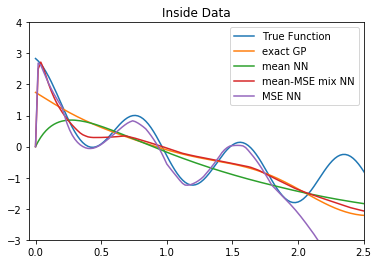
\includegraphics[scale=.85]{inside_data.png}
\end{frame}



\begin{frame}
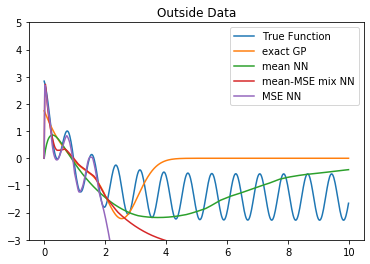
\includegraphics[scale=.85]{outside_data.png}
\end{frame}











\begin{frame}
\frametitle{Approximating Posterior Gaussian Processes}
\begin{rem}
Focusing on $h_{\eta}$, let $(s_k, t_l)_{k,l}^{a,b}$ be a grid of $T^2$. Using the triangle inequality like before, except now adding a symmetric penalty term, we obtain an $l^1$ loss function given by
\begin{align*}
        l_1(\eta) 
    &= \frac{1}{ab} \sum\limits_{k=1}^a \sum\limits_{l=1}^b  \bigg [ \sum\limits_{j=1}^n |h_{\eta}(x_j, t_l) - c(x_j, t_l)| c(s_k, x_j)   \\
    & \hspace{2.5cm} + \sig^{2}  |h_{\eta}(s_k, t_l)| \bigg] \\
    &  + \frac{1}{ab} \sum\limits_{k=1}^a \sum\limits_{l=1}^b |c(s_k, t_l) - c(t_l, s_k)|
    \end{align*}
\end{rem}

\end{frame}














\begin{frame}
\frametitle{Approximating Posterior Gaussian Processes}
\begin{rem}
Using the Jensen's inequality like before, except now adding a symmetric penalty term, we obtain an $l^2$  loss function given by
\begin{align*}
        l_2(\eta) 
        &= \frac{1}{ab} \sum\limits_{k=1}^a \sum\limits_{l=1}^b  \bigg [ \bigg(\sum\limits_{j=1}^n (h_{\eta}(x_j, t_l) - c(x_j, t_l)) c(s_k, x_j) \bigg)^2   \\
    & \hspace{2.5cm} + \sig^{2}  h_{\eta}(s_k, t_l)^2 \bigg] \\
        &+ \frac{1}{ab} \sum\limits_{k=1}^a \sum\limits_{l=1}^b (c(s_k, t_l) - c(t_l, s_k))^2
    \end{align*}
\end{rem}

\end{frame}

















\begin{frame}
\section{References}
\frametitle{References}

\begin{itemize}
\item \href{https://github.com/carsonaj/Mathematics/blob/master/Introduction\%20to\%20Analysis/Introduction\%20to\%20Analysis.pdf}{analysis notes}

\item \href{https://github.com/carsonaj/Mathematics/blob/master/Introduction\%20to\%20Measure\%20and\%20Integration/Introduction\%20to\%20Measure\%20and\%20Integration.pdf}{integration notes}

\item \href{https://en.wikipedia.org/wiki/Reproducing_kernel_Hilbert_space}{RKHS's}

\item \href{https://en.wikipedia.org/wiki/Representer_theorem}{Representer Theorem}
\end{itemize}




\end{frame}


\end{document}